
\pbn
\section{Decision making at the margin}

%\paragraph{Learning objectives}	By the end of this section, you will be able to:
%\itex{\item Calculate total utility
	%	\item Propose decisions that maximize utility
	%	\item Explain marginal utility and the significance of diminishing marginal utility}

%\subsection{A rule for maximizing utility}
\subsection{Total utility and diminishing marginal utility}
To understand how a household will make its choices, economists look at what consumers can afford, as shown in a budget constraint line, and the total utility or satisfaction derived from those choices. In a budget constraint line, the quantity of one good is measured on the horizontal axis and the quantity of the other good is measured on the vertical axis. The budget constraint line shows the various combinations of two goods that are affordable given consumer income. Consider the situation of Jose, shown in the following figure Jose likes to collect T-shirts and watch movies.

A Choice between Consumption Goods. Jose has income of \$56. Movies cost \$7 and T-shirts cost \$14. The points on the budget constraint line show the combinations of movies and T-shirts that are affordable.

\begin{center}
	\includegraphics[width=0.5\linewidth]{../../../pic/micro/jose}
\end{center}


\pbn
Jose wishes to choose the combination that will provide him with the greatest \textbf{utility}, which is the term economists use to describe a person's level of satisfaction or happiness with his or her choices.

The table below shows how Jose’s utility is connected with his consumption of T-shirts or movies. The most common pattern of total utility, as shown here, is that consuming additional goods leads to greater total utility, but at a decreasing rate. The third column shows marginal utility, which is the additional utility provided by one additional unit of consumption. This equation for marginal utility is:
\[
MU=\frac{\textnormal{change in total utlity}}{\textnormal{change in quantity}}
\]

Notice that marginal utility diminishes as additional units are consumed, which means that each subsequent unit of a good consumed provides less additional utility. This is an example of the law of diminishing marginal utility, which holds that the additional utility decreases with each unit added.

\pbn
\subsection{Calculating total utility}
The question now is how can he maximize his utility? Well, in this case Jose has only five different options because it does not make sense to consume half of a t-shirt. Thus, we simply need to calculate for each of these option his overall utility and go for the highest number which is in point S.
\begin{center}
	\includegraphics[width=0.5\linewidth]{../../../pic/micro/jose2}
\end{center}

\pbn
\subsection{Marginal utility per unit of money}
Another way to look at this is by focusing on satisfaction per dollar. In other words, the \textbf{marginal utility per dollar} is the amount of additional utility Jose receives given the price of the product. 
\[
\textnormal{marginal utility per dollar}=\frac{\textnormal{marginal utility}}{\textnormal{price}}
\]
For Jose’s T-shirts and movies, the marginal utility per dollar is shown in \autoref{tab:jose3}.
\begin{table}[h]
	\caption{Marginal utility and consumers' decision}\label{tab:jose3}
	\begin{center}
		\includegraphics[width=0.8\linewidth]{../../../pic/micro/jose3}
	\end{center}
	\note{The table stems from \cite{Shapiro2022Principles}.}
\end{table}


Jose's first purchase will be a movie because it gives him the highest marginal utility per dollar and it is affordable. Jose will keep purchasing movies because they give him a greater \textit{bang or the buck} until the sixth movie is equivalent to a T-shirt purchase. So he will choose to purchase six movies and one T-shirt.

\exex{Error in table}{In \autoref{tab:jose3} is an error. Can you find it?}

\boxx{\textbf{A rule for maximizing utility}
	This way to come to the optimal choice can be written as a general rule: the utility-maximizing choice between consumption goods occurs where the marginal utility per dollar is the same for both goods:
	\begin{align*}
		\textnormal{marginal utility per dollar of good 1}&=\textnormal{marginal utility per dollar of good 2}\\
		\frac{22}{14}&=\frac{11}{7}\\
		1.6&=1.6
\end{align*}}

%---------------------------

\pbn
\section{Consumption and production choices}\label{consumption-and-production-choices}

In microeconomics, utility maximization (in its simplest form when having just two goods) involves selecting a combination of two goods that satisfies two essential conditions, see figure \ref{fig:optimalconsumption}:

\begin{enumerate}
	\item
	The chosen point of utility maximization must fall within the attainable region defined by the Production Possibility Frontier (PPF) or be affordable within the constraints of a given budget.
	\item
	The selected point of utility maximization must lie on the highest indifference curve that is consistent with the first condition.
\end{enumerate}

\begin{figure}
	\centering
	\includegraphics[width=0.5\textwidth]{pic/optimalconsumption.png}
	\caption{\label{fig:optimalconsumption} Optimal production choice and the terms of trade}
\end{figure}

These conditions ensure that the consumer selects the optimal bundle of goods that maximizes their utility while taking into account the constraints imposed by production capabilities or budget limitations.

By analyzing production possibilities and individual preferences, economists gain insights into how consumers make choices, allocate resources, and achieve utility maximization. Understanding these concepts helps economists explore the trade-offs and decision-making processes that influence consumer behavior and shape market dynamics.

%If you are not familiar with the basic principles of the production possibility frontier curve, indifference curves, and budget constraints, I recommend referring to section \ref{micro-pre} of the appendix for a comprehensive overview. This section provides a detailed explanation and exploration of these concepts.


\subsection{The role of income and budget}\label{the-role-of-income-and-budget}

If income increases the budget constraint curve shifts outwards (to the right) as shown in figure \ref{fig:incomechange}.



The utility-maximizing choice on the original budget constraint is M. The dashed horizontal and vertical lines extending through point M allow you to see at a glance whether the quantity consumed of goods on the new budget constraint is higher or lower than on the original budget constraint. On the new budget constraint, a choice like N will be made if both goods are \emph{normal goods}. If good \(x\) is an \emph{inferior good}, a choice like P will be made. If good \(y\) is an \emph{inferior good}, a choice like Q will be made.

\begin{figure}
	\centering
	\includegraphics[width=0.5\textwidth]{pic/incomechange.png}
	\caption{\label{fig:incomechange} Impact of income change on consumption}
\end{figure}

\subsection{The role of prices}\label{the-role-of-prices}
When the price rises, the budget constraint shifts inwards for the good that becomes more expensive. For example, in \autoref{fig:pricechange} good x doubles in price and hence the budget line shifts inwards and the old consumption point M is not attainable anymore. The dashed line make it possible to see at a glance whether the new consumption choice involves less of both goods, or less of one good and more of the other. The new possible choices would be good \(x\)'s and more good \(y\)'s, like point H, or less of both goods, as at point J. Choice K would mean that the higher price of good \(x\) led to exactly the same quantity of good \(x\) being consumed, but fewer of good \(y\). Choices like L are theoretically possible (if good \(x\) are giffen goods) but highly unlikely in the real world, because that would mean that a higher price for goods \(x\) means a greater quantity consumed of good \(x\).

\begin{figure}
	\centering
	\includegraphics[width=0.5\textwidth]{pic/pricechange.png}
	\caption{\label{fig:pricechange} Impact of price change on consumption}
\end{figure}


\subsection{Substitution and income effect}\label{substitution-and-income-effect}

When prices increase, individuals typically respond by reducing their consumption of the product with the higher price. This reaction is driven by two factors, both of which can occur simultaneously.

\begin{figure}
	\centering
	\includegraphics[width=1\textwidth]{pic/hicksdecomp}
	\caption{\label{fig:hicksdecomp} Impact of income change on consumption}
\end{figure}

The \emph{substitution effect} occurs when a price change incentivizes consumers to consume less of a good with a relatively higher price and more of a good with a relatively lower price.

The \emph{income effect} stems from the fact that a higher price effectively reduces the purchasing power of income (even if actual income remains the same). This reduction in purchasing power leads to a decrease in the consumption of the good, particularly when the good is considered normal.

Figure \ref{fig:hicksdecomp} illustrates the Hicksian decomposition for a price reduction of good \(A\), which affects the consumption of goods \(A\) and \(B\), shifting the consumption point from \(C\) to \(D\). The point \(C'\) represents the hypothetical consumption point resulting from a rotated budget constraint that reflects the new price relationship.

\exex{The graphical foundations of demand curves}{
	
	A shift in the budget constraint means that when individuals are seeking their highest utility, the quantity that is demanded of that good will change. In this way, the logical foundations of demand curves---which show a connection between prices and quantity demanded---are based on the underlying idea of individuals seeking utility.
	
	In Figure \ref{fig:tpoc}, two points of consumption are displayed, illustrating the optimal choices made by customers when faced with prices \(p_x^1>p_x^2\). The objective of this exercise is to graphically derive the demand function for good \(x\). To accomplish this, please provide a second two-dimensional plot below the existing graph, with the price of good \(x\), \(p_x\), represented on the y-axis.
}

\begin{figure}
	\centering
	\includegraphics[width=1\textwidth]{pic/twopointsofconsumption.png}
	\caption{\label{fig:tpoc} Graphical derivation of the demand function}
\end{figure}

%\exex{Derivation of demand function using the Lagranian multiplier}{
	%	
	%	A representative consumer has on average the following utility function:
	%	\(U=x y,\) and faces a budget constraint of \(B=P_{x} x+P_{y} y,\) where \(B, P_{x}\)
	%	and \(P_{y}\) are the budget and prices, which are given. Solve the following choice problem:
	%	
	%	Maximize \(U=x y\) s.t. \(B=P_{x} x+P_{y} y\).
	%	
	%	Please find solution to the exercise \protect\hyperlink{sol:derofdemand}{in the appendix.}
	%}
%
%\exex{	Cobb-Douglas and demand}{\label{exr:cdanddemand}
	%	
	%
	%	
	%	A consumer who has a Cobb-Douglas utility function \(u(x, y)=A x^{\alpha} y^{\beta}\)
	%	faces the budget constraint \(p x+q y=I\), where \(A, \alpha, \beta, p,\) and \(q\) are
	%	positive constants.
	%	Solve the problem:
	%	
	%	\[
	%	\begin{array}{lll}
		%		\max A x^{\alpha} y^{\beta} & \text { subject to } & p x+q y=I
		%	\end{array}
	%	\]
	%	
	%	Please find solution to the exercise \protect\hyperlink{sol:cdanddemand}{in the appendix.}
	%}

\subsection{Consumption, production, and terms of trade}\label{consumption-production-and-terms-of-trade}

Market prices in a closed economy:
The price relation of two goods, the so-called terms of trade, is determined by the slope of the Production Possibility Frontier (PPF) at the point where it is tangent to the indifference curve. This relationship highlights the trade-off between the two goods and their relative scarcity within a closed economy.

Utility maximizing production:
The production point that maximizes utility is where the PPF is tangent to the price relation, i.e.~the \emph{terms of trade}. This principle applies not only in a closed economy (autarky) but also under free trade (open economy). It implies that producers should allocate resources in a way that balances the trade-off between producing more of one good at the expense of another, while considering consumer preferences. Figure \ref{fig:optimalconsumption} depicts this.




\exex{Understanding indifference curves and budget constraints}{
	
	
	\begin{enumerate}
%		\item
%		Which indifference curve in the figure on the right represents the highest utility level? Explain your decision.
		\item
		Suppose two goods are perfect substitutes\footnote{Two goods are substitutes if they can be used for the same purpose or provide the same utility to the consumer}. Draw the indifference curves for perfect substitutes.
		\item
		Suppose two goods are perfect complements\footnote{Two goods are complements if they go well together and the demand for one good is related to the demand for another good. A perfect complement is a good that must be consumed together with another good}. Draw the indifference curves for perfect complements.
		\item
		Suppose you have a fixed income \(I=10\) that you can spend on consuming two goods \(x, y\) at certain prices \(p_x=1, p_y=1\). Draw the budget line consisting of all possible combinations of two goods that a consumer can buy at certain market prices by allocating his income. Using indifference curves, sketch what each consumer should consume to maximize utility.
	\end{enumerate}
	
	%	Please find solution to the exercise \protect\hyperlink{sol:Uic}{in the appendix.}
}

\begin{figure}
	\centering
	\includegraphics[width=0.5\textwidth]{pic/utility-max.jpg}
	\caption[\label{fig:utilmax} Utility maximization]{\label{fig:utilmax} Utility maximization}
	\note{This graph is taken from \citet[ch.~4]{Emerson2020Intermediate}}	
\end{figure}



\solx{Understanding indifference curves and budget constraints}{\label{sol:Uic}
	\begin{enumerate}
		\item
		\(IC_3\) represents the highest level of utility. \(IC_1\) represents the lowest level of utility.\\
		\item
		Task solved in class.
		\item
		Task solved in class.
		\item
		The budget line can be sketched into a y-x plot by solving \(p_xx+p_yy=I\) for y: \[y=\frac{I}{p_y}-\frac{p_x}{p_y}x\]
	\end{enumerate}
}

\exex{Utility maximization}{
	Figure \ref{fig:utilmax} stems from \citet[ch.~4]{Emerson2020Intermediate}. Use the following sentences to describe the respective points in the figure.
	
	\begin{itemize}
		\item
		Optimal bundle.
		\item
		Can do better by trading some B for some A.
		\item
		Can do better by trading some B for some A.
		\item
		Unaffordable.
	\end{itemize}
	
	Please find solutions to the exercise in \citet[ch.~4]{Emerson2020Intermediate}.
}

\exex{Burgers and drinks}{
	Suppose you are in a fast food restaurant and you want to buy burgers and some drinks. You have \euro 12 to spend, a burger costs \euro 3 and a drink costs \euro 2.
	\abcx{
		\item Assume that you want to spend all your money and that you can only buy complete units of each products. What are the possible choices of consumption?
		\item Given your utility function $U(x,y)=B^{0.6}D^{0.4}$ calculate for each possible consumption point your overall utility. How will you decide?
		\item Assume that you want to spend all your money and that both products can be bought on a metric scale where one burger weights 200 grams and a drink is 200 ml. How much of both goods would you consume now? \textit{Hint: Use the Lagrangian multiplier method.}\footnote{Also see: \url{http://www.sfu.ca/~wainwrig/5701/notes-lagrange.pdf}}
}}

\pbn
\solx{Burgers and drinks}{
	\abcx{
		\item In the plot, I marked all 19 possible bundles of burger and drinks of consumption.  The budget constraint is shown by the solid line.
		
		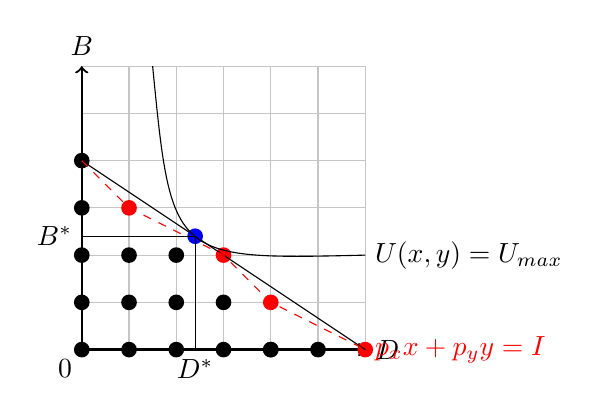
\begin{tikzpicture}[scale=0.6] 
			\draw [color=gray!50,opacity=0.9]  [step=10mm] (0,0) grid (6,6);
			
			\draw[thick,<->] (0,6) node[above]{$B$}--(0,0)--(6,0) node[right]{$D$};
			
			\node [below left] at (0,0) {$0$};
			\node at (1,1)[circle,fill,inner sep=2pt]{};
			\node at (1,2)[circle,fill,inner sep=2pt]{};	
			\node[red] at (1,3)[circle,fill,inner sep=2pt]{};
			\node at (2,1)[circle,fill,inner sep=2pt]{};
			\node at (3,1)[circle,fill,inner sep=2pt]{};
			\node[red] at (4,1)[circle,fill,inner sep=2pt]{};
			\node at (2,2)[circle,fill,inner sep=2pt]{};
			\node[red] at (3,2)[circle,fill,inner sep=2pt]{};
			
			\node at (0,1)[circle,fill,inner sep=2pt]{};
			\node at (0,2)[circle,fill,inner sep=2pt]{};
			\node at (0,3)[circle,fill,inner sep=2pt]{};
			\node at (2,0)[circle,fill,inner sep=2pt]{};
			\node at (3,0)[circle,fill,inner sep=2pt]{};
			\node at (4,0)[circle,fill,inner sep=2pt]{};
			\node at (0,4)[circle,fill,inner sep=2pt]{};
			\node at (4,0)[circle,fill,inner sep=2pt]{};
			\node at (5,0)[circle,fill,inner sep=2pt]{};
			\node at (0,0)[circle,fill,inner sep=2pt]{};
			\node[red] at (6,0)[circle,fill,inner sep=2pt]{};
			\node at (1,0)[circle,fill,inner sep=2pt]{};
			\draw(0,4) -- (6,0);
			\draw[dashed,red](0,4) -- (1,3) -- (3,2) -- (4,1) -- (6,0) node[right]{$p_xx+p_yy=I$};
			\node[blue] at (2.4,2.4)[circle,fill,inner sep=2pt]{};
			%\node at (1,3)[circle,fill,inner sep=2pt]{};
			
			\node [below] at (2.4,0) {$D^{*}$};
			%	
			\node [left] at (0,2.4) {$B^{*}$};
			
			%	\draw(1,9)--(9,1) node[right]{$p_xx+p_yy=I$};
			%	
			\draw(0,2.4)--(2.4,2.4)--(2.4,0);
			%	
			\draw(1.5,6) ..controls (1.9,1.9)  .. (6,2) node[right]{$U(x,y)=U_{max}$};
			
		\end{tikzpicture}
		\item We now should calculate the utility of all 19 points but only the red dots denote choices that may yield an optimal utility. The best utility is at when we buy 2 burger and 3 drinks: $$U=2^{.6}3^{.4}=2.35$$
		\item Solve: 
		$$
		\mathcal{L}=B^{0.6}D^{0.4}-\lambda(12-3B-2D)
		$$
		FOC: 
		\begin{align*}
			12-3B+2D&=0\\
			.6B^{-0.4}D^{0.4}+3\lambda&=0\\
			.4B^{0.6}D^{-0.6}+2\lambda&=0
		\end{align*}
		Solving the second and third FOC for $\lambda$, substituting $\lambda$ gives:
		$$B=D$$
		which we can plug in the first FOC to get
		$$B^*=2.4 \quad \text{and} \quad D^*=2.4$$
	}
	
}





\section{Consumption choice using the Lagrangian Multiplier}

In exercise \ref{exe:Burgers and drinks} we have seen a method how to make a optimal consumption decision when the numbers of bundles of goods is finite. However, if there is an infinite amount of possibilities a consumer could choose, we need a more advanced method, the Lagrangian Multiplier Method.

\pbn
\subsection{Lagrangian Multiplier Method}
The method is a strategy for finding the local maxima and minima of a function subject to constraints.\footnote{For a detailed mathematical explanation, feel free to watch Aviv Censor's video \websmall\url{https://youtu.be/AxEVJoxv-Z8}.}

\begin{minipage}{0.3\textwidth}
	\begin{center}
		\includegraphics[width=0.8\linewidth]{../../../pic/cla/Lagrange}
		Joseph-Louis Lagrange (1736-1813)
	\end{center}
\end{minipage}
\begin{minipage}{0.7\textwidth}
	\begin{center}
		\includegraphics[width=0.8\linewidth]{../../../pic/cla/lagr2}
	\end{center}
\end{minipage}
The red curve shows the constraint $g(x, y) = c$. The blue curves are contours of $f(x, y)$. The point where the red constraint tangentially touches a blue contour is the maximum of $f(x, y)$ along the constraint, since $d1 > d2$.


\begin{figure}[h]
	\begin{center}
		\includegraphics[width=0.6\linewidth]{../../../pic/micro/lagrange-yt}
		\note{\tv \url{https://youtu.be/8mjcnxGMwFo}} \textit{Lagrange Multipliers | Geometric Meaning \& Full Example}
	\end{center}
	\caption{Lagrange Multiplier graphically explained}\label{fig:lagrange-yt}
\end{figure}


\boxx{
	\paragraph{Step 1: The problem to be solved}
	The problem that we want to solve can be written in the following way,
	$$
	\begin{array}{ll}
		\max _{x, y} & F(x, y) \\
		\text { s.t. } & g(x, y)=0
	\end{array}
	$$
	where $F(x, y)$ is the function to be maximized and $g(x, y)=0$ is the constraint to be respected. 
	Notice that $\max _{x, y}$ means that we must solve (maximize) with respect to $x$ and $y$.
	
	\paragraph{Step 2: Define the Lagrangian Multiplier}
	Define a new function, the \textit{Lagrangian} $\mathcal{L}$, by combining the two functions of the problem and adding the new variable $\lambda$. The $\lambda$ is called the \textit{Lagrange Multiplier}.
	$$
	\mathcal{L}(x, y, \lambda)=F(x, y)-\lambda g(x, y)
	$$
	
	\paragraph{Step 3: Find the first order conditions}
	Differentiate $\mathcal{L}$ w.r.t. $x, y,$ and $\lambda$ and equate the partial derivatives to 0:
	\begin{align*}
		\frac{\partial \mathcal{L}(x, y, \lambda)}{\partial x}=0 & \Leftrightarrow \frac{\partial F(x, y)}{\partial x}-\lambda \frac{\partial g(x, y)}{\partial x}=0 \\
		\frac{\partial \mathcal{L}(x, y, \lambda)}{\partial y}=0 & \Leftrightarrow \frac{\partial F(x, y)}{\partial y}-\lambda \frac{\partial g(x, y)}{\partial y}=0 \\
		\frac{\partial \mathcal{L}(x, y, \lambda)}{\partial \lambda}=0 & \Leftrightarrow g(x, y)=0
	\end{align*}
	
	\paragraph{Step 4: Solve the system of equations}
	The solution to the system of three equations above gives the required optimal quantities.
}


\pbn
\exex{Consumption Choice}{
	Suppose you want to spend your complete budget of \euro 30, $$I=30,$$ on the consumption of two goods, $A$ and $B$. Further assume good $A$ costs \euro 6, $$p_A=6,$$ and good $B$ costs \euro 4, $$p_B=4$$ and that you want to maximize your utility that stems from consuming the two goods.
	Calculate how much of both goods to buy and consume, respectively, when your utility function is given as  $$U(A,B)=A^{0.8}B^{0.2}$$
}

\pbn
\solx{Consumption Choice}{
	\begin{align*}
		\mathcal{L}&=A^{0.8}B^{0.2}-\lambda(30-6A-4B)\\
		FOC: \frac{\partial \mathcal{L}}{\partial \lambda}&=30-6A-4B=0 \qquad (*)\\
		\frac{\partial \mathcal{L}}{\partial A}&=0.8A^{-0.2}B^{0.2}+6\lambda=0 \qquad (**)\\
		\frac{\partial \mathcal{L}}{\partial B}&=0.2A^{0.8}B^{-0.8}+4\lambda=0 \qquad (***)
	\end{align*}
	System of 3 equation with 3 unknowns can be solved in various ways. The easiest way is to solve (**) and (***) for $\lambda$ and substitute it out:
	\enux{
		\item solve for $\lambda$
		\begin{align*}
			- \frac{2}{15} A^{-0.2}B^{0.2}&=\lambda \qquad (**')\\
			- \frac{1}{20} A^{0.8}B^{-0.8}&=\lambda \qquad (***')\\
		\end{align*}
		\item set both equations equal by substituting $\lambda$ and solve for $B$
		\begin{align*}
			\frac{2}{15} A^{-0.2}B^{0.2}&=	\frac{1}{20} A^{0.8}B^{-0.8}\\
			B&=0.375A \qquad (****) %\\
			%\Leftrightarrow B&=\frac{3}{8}A
		\end{align*}
		\item Now, plug in $(****)$ into $(*)$ to get a number for $A$
		\begin{align*}
			30&=6A+4\cdot 0.375 A\\
			\Leftrightarrow 30&=7.5A\\
			\Leftrightarrow A&=4
		\end{align*}
		\item Use $A=4$ in $(*)$ to get a number for $B$
		\begin{align*}
			30&=6\cdot 4+4 B\\
			\Leftrightarrow 6&=4B\\
			B&=\frac{6}{4}=1.5
		\end{align*}
	}
	Thus, we'd consume 4 units of good A and 1.5 of good B.
}

\pbn
\exex{Derivation of Demand Function}{
	A representative consumer has on average the following utility function: $U=x y,$ and faces a budget constraint of $B=P_{x} x+P_{y} y,$ where $B, P_{x}$ and $P_{y}$ are the budget and prices, which are given. Solve the following choice problem:\\
	Maximize $U=x y$ s.t. $B=P_{x} x+P_{y} y$.
}


%\pagebreak
\exex{Cobb-Douglas and Demand}{
	A consumer who has a Cobb-Douglas utility function $u(x, y)=A x^{\alpha} y^{\beta}$ faces the budget constraint $p x+q y=I$, where $A, \alpha, \beta, p,$ and $q$ are positive constants. Solve the consumer's problem:
	$$
	\begin{array}{lll}
		\max A x^{\alpha} y^{\beta} & \text { subject to } & p x+q y=I
	\end{array}
	$$
}

\pbn
\solx{Derivation of Demand Function}{
	The Lagrangian for this problem is
	$$
	Z=x y+\lambda\left(B-P_{x} x-P_{y} y\right)
	$$
	The first order conditions are
	$$
	\begin{array}{l}
		Z_{x}=y-\lambda P_{x}=0 \\
		Z_{y}=x-\lambda P_{y}=0 \\
		Z_{\lambda}=B-P_{x} x-P_{y} y=0
	\end{array}
	$$
	Solving the first order conditions yield the following solutions
	$$
	x^{M}=\frac{B}{2 P_{x}} \quad y^{M}=\frac{B}{2 P_{y}} \quad \lambda=\frac{B}{2 P_{x} P_{y}}
	$$
	where $x^{M}$ and $y^{M}$ are the consumer's demand functions.
}


\pbn
\solx{Cobb-Douglas and Demand}{
	The Lagrangian is
	$$
	\mathcal{L}(x, y)=A x^{\alpha} y^{\beta}-\lambda(p x+q y-I)
	$$
	Therefore, the first-order conditions are
	$$
	\begin{aligned}
		\mathcal{L}_{x}^{\prime}(x, y)=A \alpha x^{\alpha-1} y^{\beta}-\lambda p &=0 \qquad (*)\\
		\mathcal{L}_{y}^{\prime}(x, y)=A x^{\alpha} \beta y^{\beta-1}-\lambda q &=0  \qquad (**)\\
		p x+q y-I &=0  \qquad (***)
	\end{aligned}
	$$
	Solving $(*)$ and $(**)$ for $\lambda$ yields
	$$
	\lambda=\frac{A \alpha x^{\alpha-1} y^{\beta-1} y}{p}=\frac{A x^{\alpha-1} x \beta y^{\beta-1}}{q}
	$$
	Canceling the common factor $A x^{\alpha-1} y^{\beta-1}$ from the last two fractions gives
	$$
	\frac{\alpha y}{p}=\frac{x \beta}{q}
	$$
	and therefore
	$$
	q y=p x \frac{\beta}{\alpha}
	$$
	Inserting this result in $(***)$ yields
	$$
	p x+p x \frac{\beta}{\alpha}=I
	$$
	Rearranging gives
	$$
	p x\left(\frac{\alpha+\beta}{\alpha}\right)=I
	$$
	Solving for $x$ yields the following \textit{demand function}
	$$
	x=\frac{\alpha}{\alpha+\beta} \frac{I}{p}
	$$
	Inserting
	$$
	p x=q y \frac{\alpha}{\beta}
	$$
	in $(***)$ gives
	$$
	q y \frac{\partial}{\beta}+q y=I
	$$
	and therefore the \textit{demand function}
	$$
	y=\frac{\beta}{\alpha+\beta}  \frac{I}{q}
	$$
}







\solx{Derivation of demand function using the Lagranian multiplier}{
	
	The Lagrangian for this problem is
	\[
	Z=x y+\lambda\left(B-P_{x} x-P_{y} y\right)
	\]
	The first order conditions are
	\[
	\begin{array}{l}
		Z_{x}=y-\lambda P_{x}=0 \\
		Z_{y}=x-\lambda P_{y}=0 \\
		Z_{\lambda}=B-P_{x} x-P_{y} y=0
	\end{array}
	\]
	
	Solving the first order conditions yield the following solutions
	
	\[
	x^{M}=\frac{B}{2 P_{x}} \quad y^{M}=\frac{B}{2 P_{y}} \quad \lambda=\frac{B}{2 P_{x} P_{y}}
	\]
	where \(x^{M}\) and \(y^{M}\) are the consumer's demand functions.
}

\solx{Cobb-Douglas and demand}{\label{sol:cdanddemand}
	
	The Lagrangian is
	\[
	\mathcal{L}(x, y)=A x^{\alpha} y^{\beta}-\lambda(p x+q y-I)
	\]
	
	Therefore, the first-order conditions are
	\[
	\begin{aligned}
		\mathcal{L}_{x}^{\prime}(x, y)=A \alpha x^{\alpha-1} y^{\beta}-\lambda p &=0 \qquad (*)\\
		\mathcal{L}_{y}^{\prime}(x, y)=A x^{\alpha} \beta y^{\beta-1}-\lambda q &=0  \qquad (**)\\
		p x+q y-I &=0  \qquad (***)
	\end{aligned}
	\]
	
	Solving \((*)\) and \((**)\) for \(\lambda\) yields
	\[
	\lambda=\frac{A \alpha x^{\alpha-1} y^{\beta-1} y}{p}=\frac{A x^{\alpha-1} x \beta y^{\beta-1}}{q}
	\]
	Canceling the common factor \(A x^{\alpha-1} y^{\beta-1}\) from the last two fractions gives
	\[
	\frac{\alpha y}{p}=\frac{x \beta}{q}
	\]
	and therefore
	\[
	q y=p x \frac{\beta}{\alpha}
	\]
	Inserting this result in \((***)\) yields
	\[
	p x+p x \frac{\beta}{\alpha}=I
	\]
	Rearranging gives
	\[
	p x\left(\frac{\alpha+\beta}{\alpha}\right)=I
	\]
	Solving for \(x\) yields the following \textit{demand function}
	\[
	x=\frac{\alpha}{\alpha+\beta} \frac{I}{p}
	\]
	Inserting
	\[
	p x=q y \frac{\alpha}{\beta}
	\]
	in \((***)\) gives
	\[
	q y \frac{\partial}{\beta}+q y=I
	\]
	and therefore the \textit{demand function}
	\[
	y=\frac{\beta}{\alpha+\beta}  \frac{I}{q}
	\]
}






\pbn
\exex{Labor and Machines}{
	Suppose you rent a factory for a month to produce as many masks as possible. After you have paid the rent, you need to decide how many machines to buy and how many workers to hire for the given month. 
	What is optimal amount of workers and machines to employ at the given month, if you assume the following: 
	\itex{
		\item $L$ denotes the number of workers
		\item $K$ denotes the number of machines
		\item $Q$ denotes the number of masks produced
		\item $p_L$ denotes the price of a worker for a month
		\item $p_K$ denotes the price of a machine for a month
		\item $B$ denotes the money you can invest in the production of masks for the next month
		\item $B=216$
		\item the production of masks can be explained by the following Cobb-Douglas production function: $Q=K^{0.4}L^{0.6}$
		\item $p_L=2$
		\item $p_K=8$
	}
}

\pbn
\solx{Labor and Machines}{
	1. Set up Lagrangian:
	$$\mathcal{L}=K^{.4}L^{.6}-216\lambda+2\lambda L+8\lambda K$$	
	2. FOC:
	\begin{align*}
		0&=.4K^{-.6}L^{.4}-8\lambda \quad (*)\\
		0&=.6K^{-.4}L^{-.4}-2\lambda \quad (**)\\
		0&=216-2L-8K \quad (***)
	\end{align*}
	3. Solving (*) and (*) for $\lambda$ and substituting $\lambda$ gives us:
	$$\frac{1}{6}L=K \quad (****)$$
	4. Plugging (****) into (***), we get
	$$0=216-2L-8\cdot(\frac{1}{6}L)\Rightarrow L=64\frac{4}{5}$$
	5. Using that result in (***) again, we get
	$$216-2\cdot 64 \frac{4}{5}+8K \Rightarrow K=10\frac{4}{5}$$
	Thus, the optimal combination of inputs is $L=64\frac{4}{5}$ and $K=10\frac{4}{5}$.
}










